\chapter{Event Reconstruction}
\label{chapter:reconstruction}

\section{Electron Reconstruction}
\label{sec:electron_reconstruction}

Reconstruction of electrons in CMS is complicated by the fact that the tracker
contains a large amount of material and so electrons must pass through up to
two radiation lengths of material before reaching ECAL. Information about the
material in front of ECAL is given in
\FIG~\ref{fig:tracker_material}\cite{cms_tracker_2014}. Electrons emit photons
when they interact with matter in a process known as bremsstrahlung. These
photons are then separated from the electron as they do not bend in the
magnetic field while the electron does. In order to accurately reconstruct the
energy of the electron, these photons must be accounted for in the final energy
sum, and this is what the electron reconstruction algorithm attempts to do.

\begin{figure}[!htbp]
    \centering
    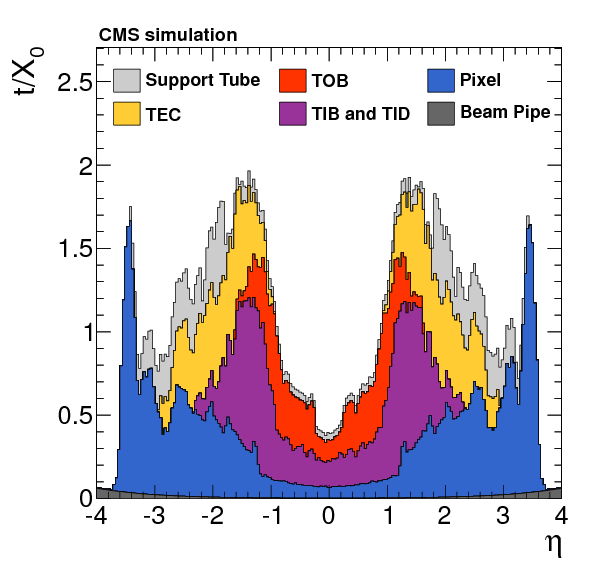
\includegraphics[width=\textwidth]{figures/tracker_material_budget.png}
    \caption[
        Material thickness infront of of ECAL.
    ]{
        The thickness of material, $t$, divided by the radiation length,
        \radiationlength, encountered by particles leaving the nominal
        interaction point before reaching ECAL.
    }
    \label{fig:tracker_material}
\end{figure}

The reconstruction of electrons with $\pt > 20 \GeV$ in CMS begins with a
``seed'' cluster of energy deposits in ECAL that has the right \TODO{shape} to be an
electron \cite{eg_reco_2010}. As an electron bends in the magnetic field, it
takes a helictical path at constant $\eta$ but changing $\phi$. Any photons
radiated by the electron will lie along this path. These photons must be added
together with the electron in order to accurately measure its energy, and so
additional clusters on the same path as the seed cluster are connected to form
a ``supercluster'' \cite{baffioni_2007}. A supercluster, therefore, includes
the energy deposit from the electron as well as the energy from its nearby
photons at constant $\eta$.

From these superclusters, a volume in the tracker where the electron is likely
to have come from is determined by propagating the energy-weighted mean
position of the supercluster back through the magnetic field. This spot is then
used to seed a track-finding algorithm in the pixel layer. Hits in the tracker
are searched for starting at the innermost layer and working outward. In order
to account for the changing shape of the track as the electron loses energy
from interacting with the tracker material, a ``Gaussian Sum Filter'' (GSF)
\cite{adam_2005} is used rather than the simpler Kalman filter used for muons
and hadrons. Low energy electrons ($\ET < 15 \GeV$) are constructed with \pt
from the tracker and \ET from ECAL. For higher energy electrons, the ECAL
energy is used without the tracker \pt to avoid issues introduced by the
possible poor fits in the tracker. The $\eta$ and $\phi$ of all electron
candidates, regardless of energy, is taken from the track by projecting back to
the interaction point.

\section{Additional Corrections}
\label{sec:corrections}

Although the measurement of \phistar is relatively insensitive to the energy of
the electrons, the energy still plays a role in determining the electron \pt
and hence whether an event passes the selection criteria used in this analysis
(discussed in \SEC~\ref{ssec:electron_selection}). Therefore, it is important
to accurately measure this quantity, even if it does not directly change the
final observable. To this end, two sets of energy and momentum corrections,
centrally produced by the CMS collaboration, are applied to both the
data and the reconstructed MC quantities. A summary of the method used to
derive these corrections follows because the papers detailing them are not
public.

\subsection{Regression}

The first set of corrections were calculated using a multivariate regression
trained on \Ztoee and \higgstoZZ MC \cite{cms_an_2012-327}. The regression used
a boosted decision tree trained on 41 different variables parameterizing
electron shower shape, the electron track, and the location of the shower in
EB. The algorithm was trained separately for EB and EE electrons. In order to
prevent over-training the MC samples were split in half, with one half used for
training and the other half used for validation. Electrons used in the
regression were required to have low radiated energy fraction ($< 0.01$) as
determined by the generator level MC and $\pt > 7 \GeV$. The target variable
was the ratio of the generator level bare electron energy over the
reconstructed energy. This correction was applied to both the data and the
reconstructed MC electrons used in this analysis.

\subsection{Energy Scale and Resolution}

The second set of corrections were calculated with \Ztoee MC using two
independent methods \cite{cms_an_2013-253}. The first method was used to
correct for the energy scale while the second method was used to correct for
the resolution.

In the first method, the MC sample and the data were fit with the convolution
of a Breit-Wigner with a Crystal Ball (CB) function. The CB function is used to
model the resolution of the detector and losses due to bremsstrahlung from the
material in front of ECAL. It consists of a Gaussian with a power-law low-side
tail. It was first used by the Crystal Ball Collaboration \cite{oreglia_1980}.
The Breit--Wigner function models the analytic shape predicted for the \Z mass
resonance. The parameters of the Breit--Wigner were fixed to the nominal values
from the Particle Data Group: $\MZ = 91.188 \GeV$, $\GammaZ = 2.495 \GeV$. The
parameters of the CB function were free parameters in the fit.

The scale correction is both time dependent and $\eta$ dependent and so fits
were performed separately in four pseudorapidity bins in various run ranges.
The peak of the CB function in data and MC were compared with the relative
shift taken as the scale correction, $\Delta P$, given by
\EQ~\ref{eq:scale_correction}.

\begin{equation} \label{eq:scale_correction}
    \Delta P = \frac{\Delta m_{\text{data}} - \Delta m_{\text{MC}}}{\MZ}
\end{equation}

In the second method, two categories of electrons are defined: showering
electrons ($\RNine < 0.94$) and non-showering electrons ($\RNine > 0.94$).
\RNine is the ratio of energy in the \threebythree square of crystals in ECAL
where the electron impacted over the energy in the supercluster and so a larger
number means a narrower shower. A probability density function (PDF) is created
using the \Ztoee MC. For each event in the PDF, the supercluster energy is
modified by applying a Gaussian multiplicative factor $1+\Delta P$ with a
standard deviation of $\Delta \sigma$, where $\Delta P$ is the scale correction
and $\Delta \sigma$ models the resolution. The resolution parameter was
selected for each of the two types of electrons, the four pseudorapidity bins,
and various run ranges using a likelihood maximization. In the EB
pseudorapidity bins, there were enough events to bin in \ET and so these
corrections are also \ET dependent.

\section{Electron Variables}
\label{sec:electron_variables}

Not everything reconstructed as an electron in CMS is a real electron. One
source of fake electrons is a process referred to as charge exchange:
$\ChargeExchange \to 2 \photon + \proton$. In this process, a charged pion
interacts with a nuclear neutron which convert to a neutral pion and a proton
where the neutral pion quickly decays to two photons. If this process happens
in ECAL, it can result in a track (from the charged
pion) pointing at a supercluster with a shape similar to a photon or electron
shower (from the two photons) which will often be reconstructed as an electron.
Another source of fake electrons is coincidence events where a photon impacts
ECAL near the track left by another charged particle.

Not every electron is equally likely to be from a \Ztoee decay; many electrons
detected in CMS come from other processes. One such process is photon
conversion, \PhotonConversion, where a photon in the presence of a nucleus
converts to two electrons. Another source of electrons is from QCD jets which
can sometimes produce an electron in their numerous decays.

There are several electron variables defined in order to allow the separation
of these lower quality and fake electrons from the electrons from \Ztoee
decays. These variables are broken down into three categories:

\begin{description}
    \item[Identification (ID):] \hfill \\
        These variables quantify how much like an electron the reconstructed
        particle looks and are used to reject fake electrons like those from
        charge exchange.
    \item[Conversion Rejection:] \hfill \\
        These variables are used to reject electrons from \PhotonConversion
        conversions.
    \item[Isolation:] \hfill \\
        These variables measures how much energy from other particles is
        deposited near the electron in the detector and are used to help reject
        electrons within jets.
\end{description}

The following subsections contain plots of some of the most important electron
variables as well as a discussion of their use in selecting electrons from
\Ztoee decays. The data shown on the plots consists of every electron candidate
in the \SingleMuon dataset with $|\eta| < 2.4$ and $\pt > 20 \GeV$. This
dataset was used because the trigger that selects events for it makes no
selection on the electron variables and therefore the electron candidates in
the set represent a sample of minimally-biased electrons. The MC electrons are
from the \MADGRAPH \DYtoll sample with the same kinematic requirements are
applied as are used on the data, with the additional requirement that the event
must contain a generator level \Ztoee decay. These selections give us a data
sample that is indicative of the general distribution of all electrons in CMS
events, while the MC sample shows what electrons look like in events this
analysis
uses.

\subsection{Identification}

The shape of the electromagnetic shower in the calorimeters is used to
discriminate between electrons and other particles. Electrons generally have
very narrow showers whereas hadronic particles have wide showers. The size of
the shower in $\eta$ is characterized by \sigmaietaieta. Charge exchange events
often have a higher \sigmaietaieta than real electrons because the proton is
can be knocked loose by the interaction and leaves a broader shower.
Comparisons of the \sigmaietaieta distributions between all electrons and for
signal electrons for both EB and EE are shown in \FIG~\ref{fig:sieie}.

\begin{figure}[!htbp]
    \centering
    \begin{subfigure}[b]{\StackedPlotWidth}
        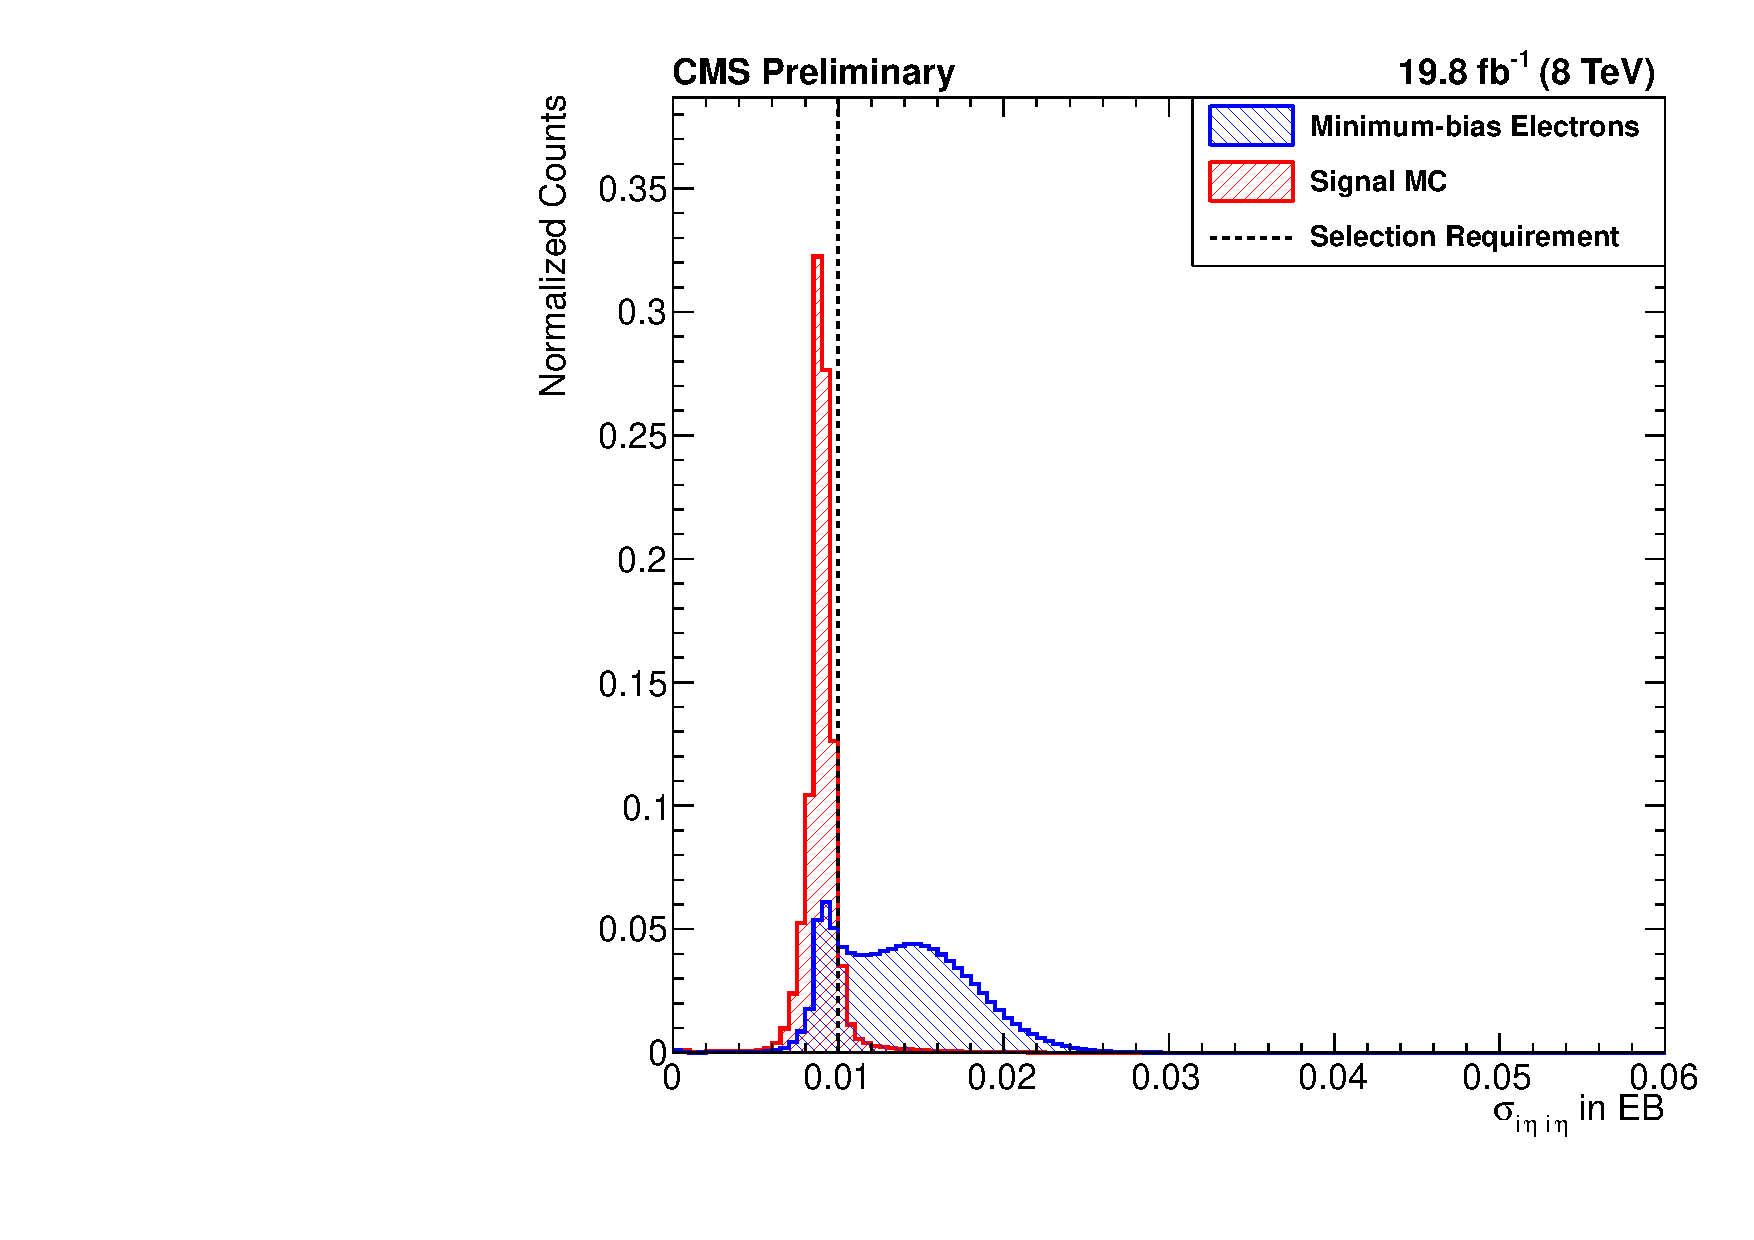
\includegraphics[width=\textwidth]{figures/e_reco_var_sigma_ieta_ieta_eb.pdf}
        \caption{}
        \label{fig:sieie_eb}
    \end{subfigure}
    \begin{subfigure}[b]{\StackedPlotWidth}
        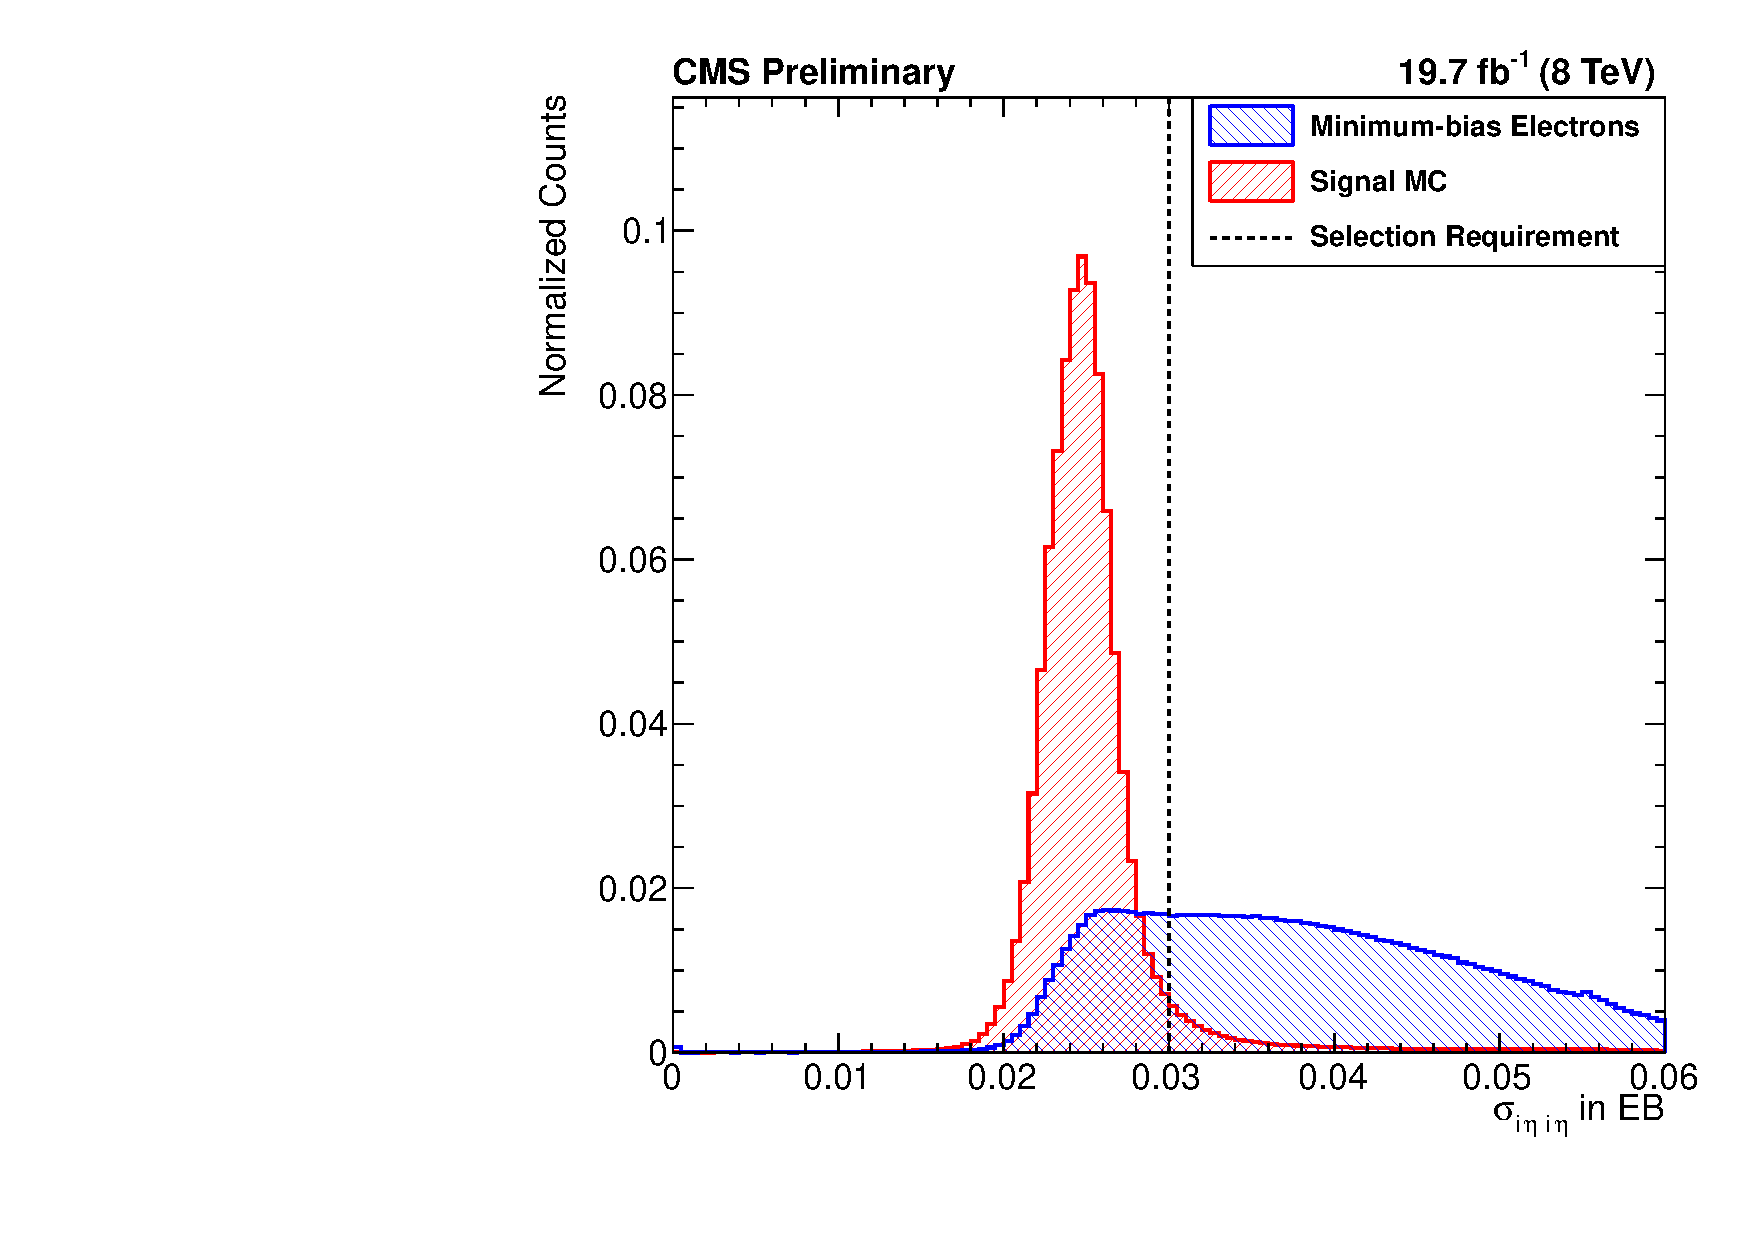
\includegraphics[width=\textwidth]{figures/e_reco_var_sigma_ieta_ieta_ee.pdf}
        \caption{}
        \label{fig:sieie_ee}
    \end{subfigure}
    \caption[
        Distributions of $\sigmaietaieta$ in EB and EE in data and MC.
    ]{
        The $\sigmaietaieta$ variable distribution in EB (top) and EE (bottom)
        for all electrons with $\pt > 20 \GeV$ and $|\eta| < 2.4$ in a set of
        events selected with a muon trigger and in \MADGRAPH \Ztoee MC.
    }
    \label{fig:sieie}
\end{figure}

Electron showers are mostly contained within ECAL and so the ratio of energy
around the hit in HCAL over the energy around the hit in ECAL, \HOverE, is also
used to parameterize the shower shape. Charge exchange events often have higher
\HOverE than electrons because the loose proton can escape and enter HCAL. A
comparison of the \HOverE distributions between all electrons and for signal
electrons is shown in \FIG~\ref{fig:he}.

\begin{figure}[!htbp]
    \centering
    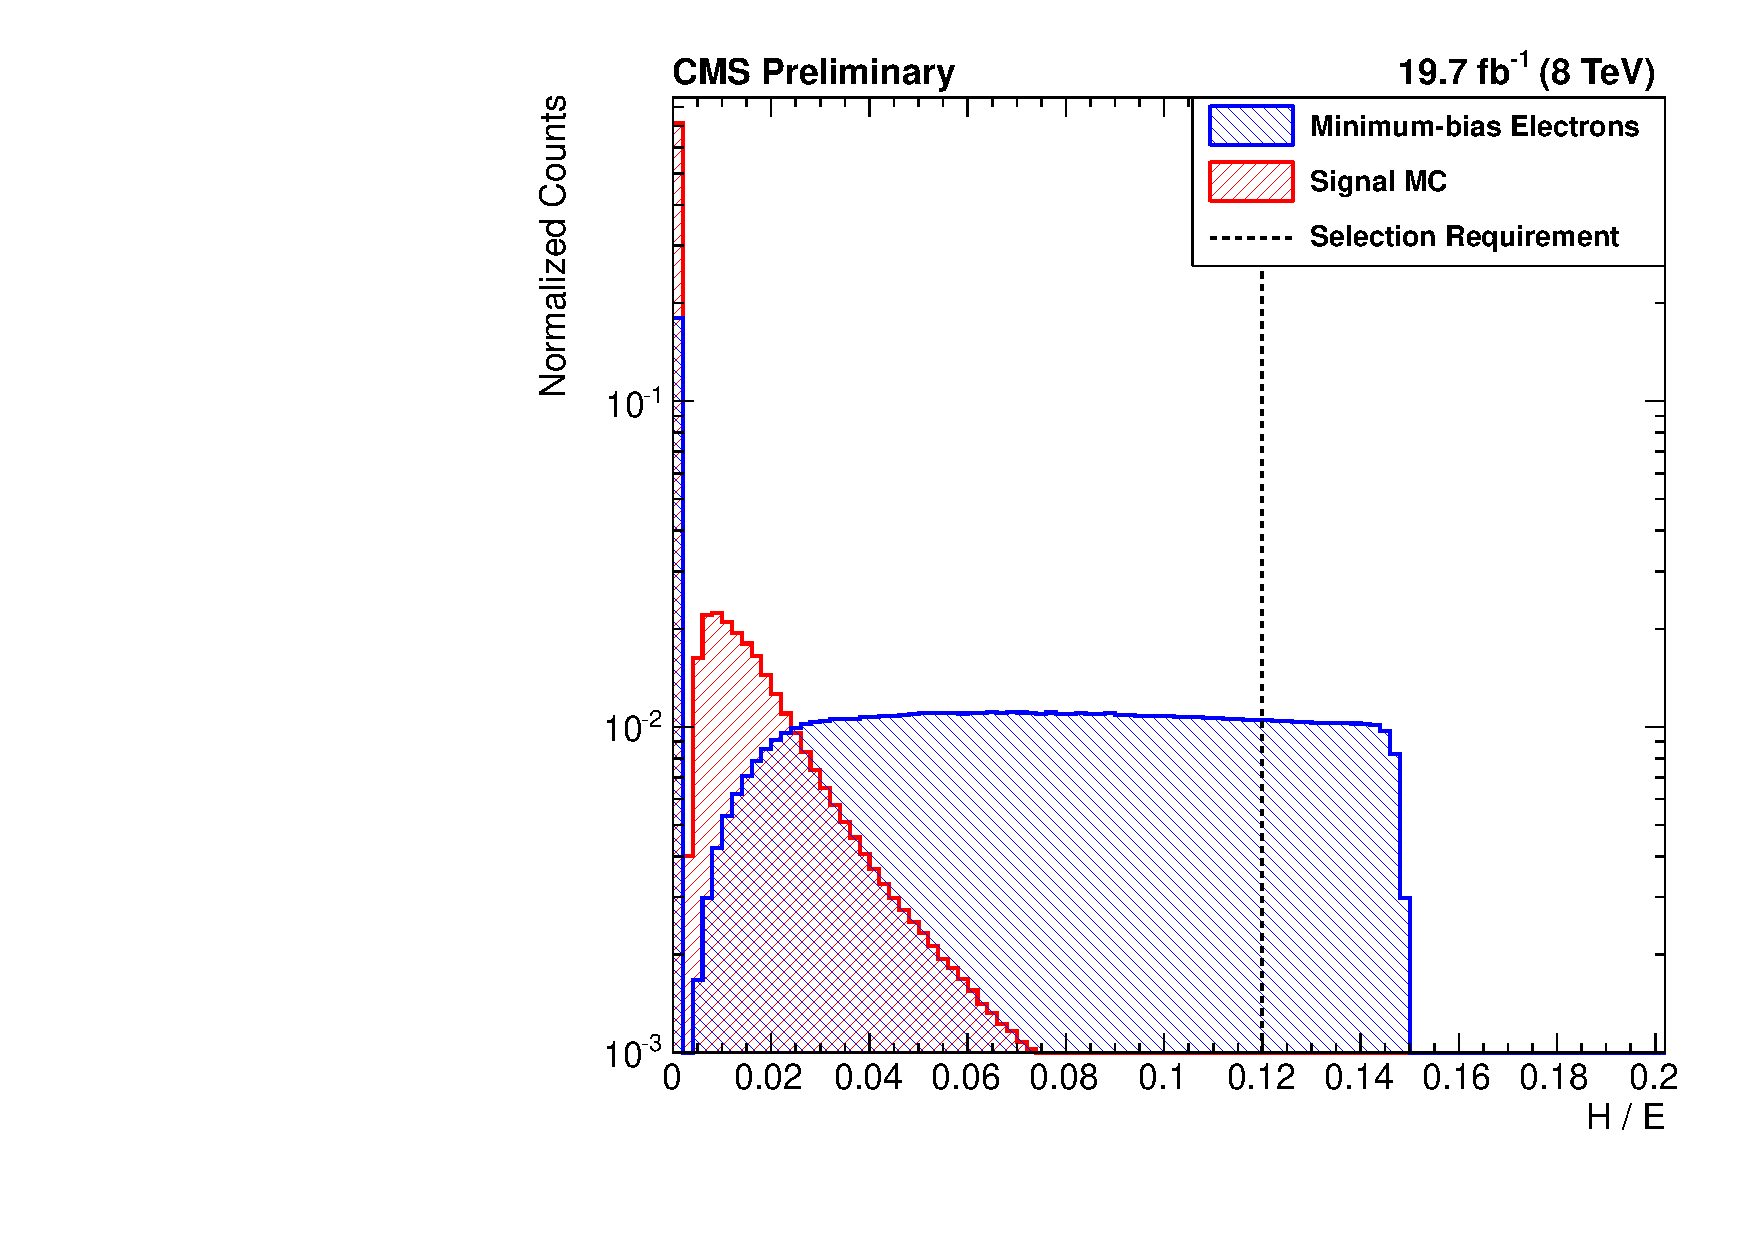
\includegraphics[width=\StackedPlotWidth]{figures/e_reco_var_he.pdf}
    \caption[
        Distributions of \HOverE in data and MC.
    ]{
        The \HOverE distributions for all electrons with $\pt > 20 \GeV$ and
        $|\eta| < 2.4$ in a set of events selected with a muon trigger and in
        \MADGRAPH \Ztoee MC.
    }
    \label{fig:he}
\end{figure}

The distance between the track and the supercluster in \coordetaphi space is
given by \dphiin and \detain. Real electrons have small values of \dphiin and
\detain because the electron caused both the track and the supercluster, but
coincidence events are equally as likely to have a large track separation as a
small one because each element comes from an independent object. Comparisons of
the \dphiin and \detain distributions between all electrons and for signal
electrons are shown in \FIGS~\ref{fig:deta} and \ref{fig:dphi}, respectively.

\begin{figure}[!htbp]
    \centering
    \begin{subfigure}[b]{\StackedPlotWidth}
        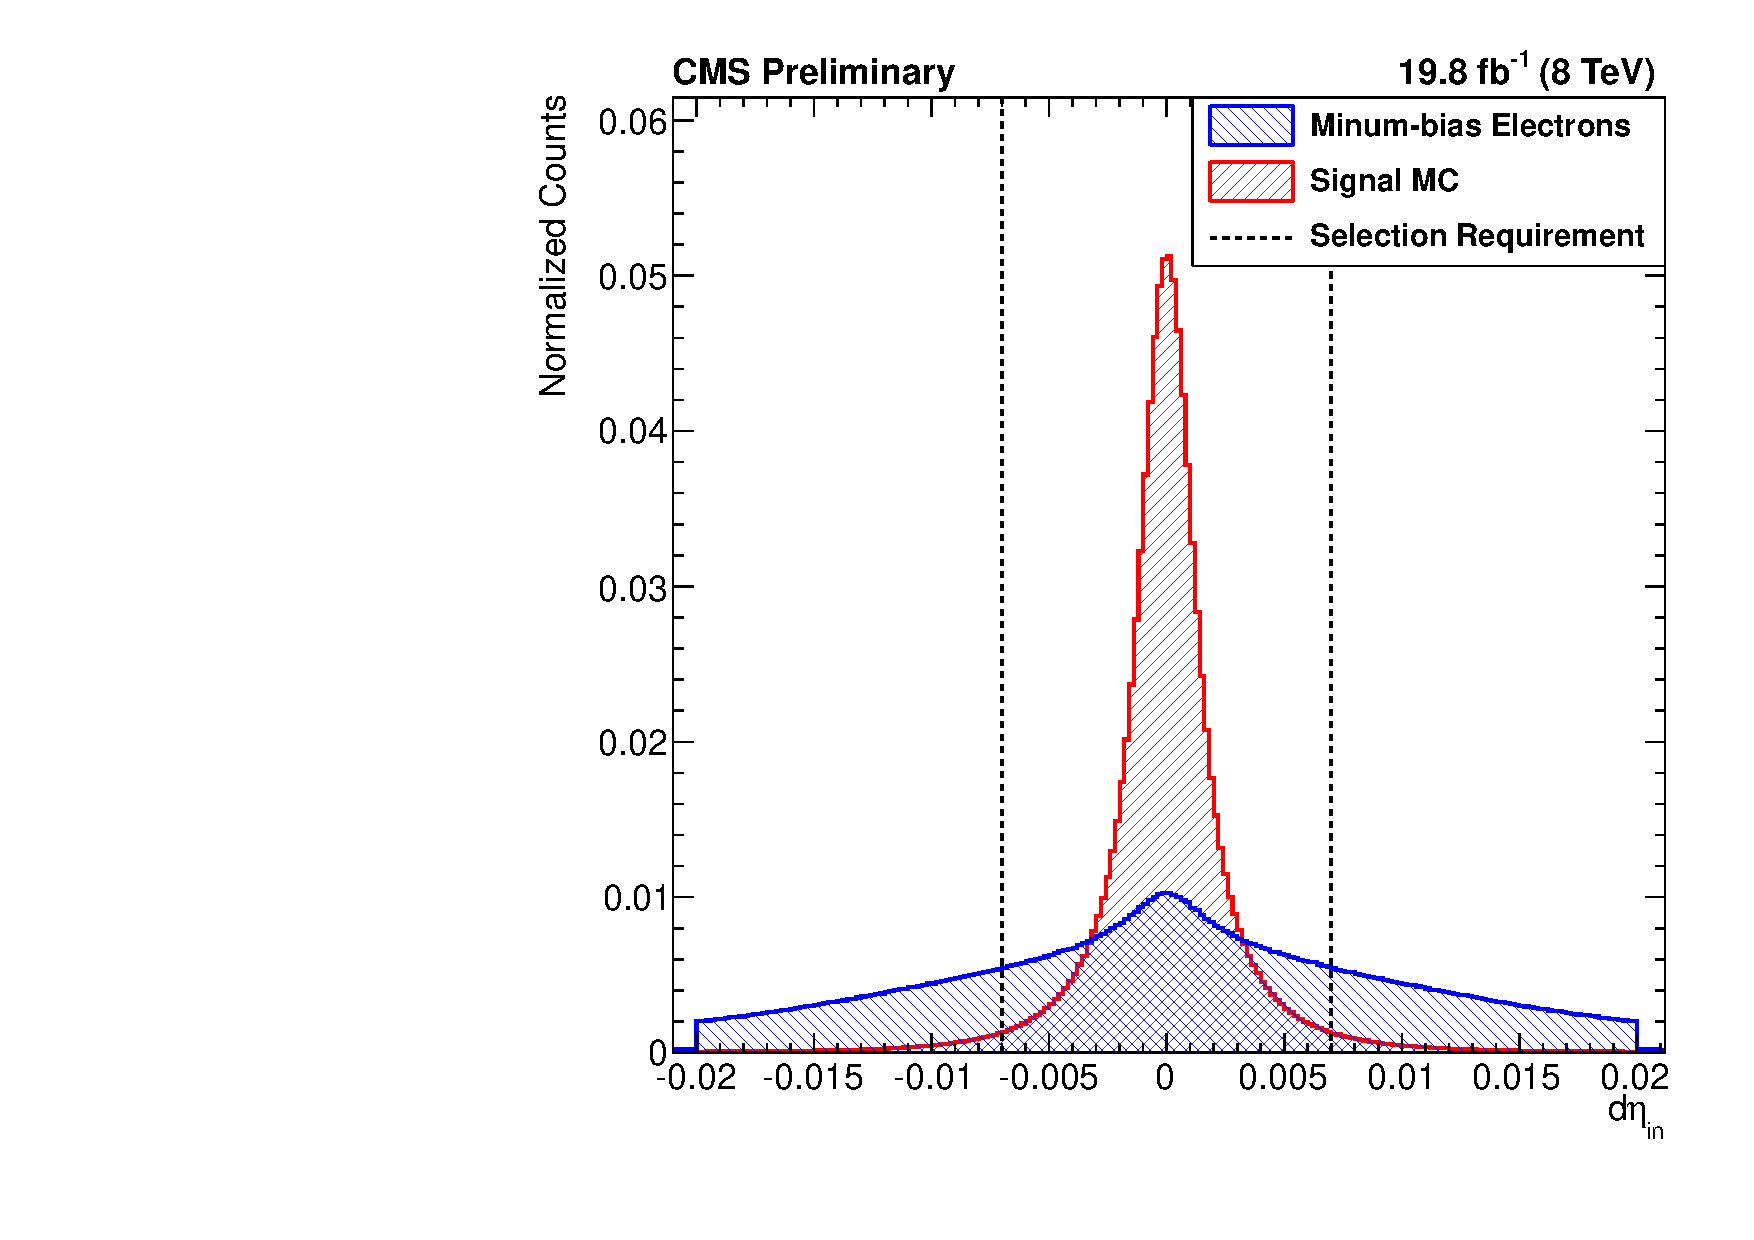
\includegraphics[width=\textwidth]{figures/e_reco_var_deta.pdf}
        \caption{}
        \label{fig:deta}
    \end{subfigure}
    \begin{subfigure}[b]{\StackedPlotWidth}
        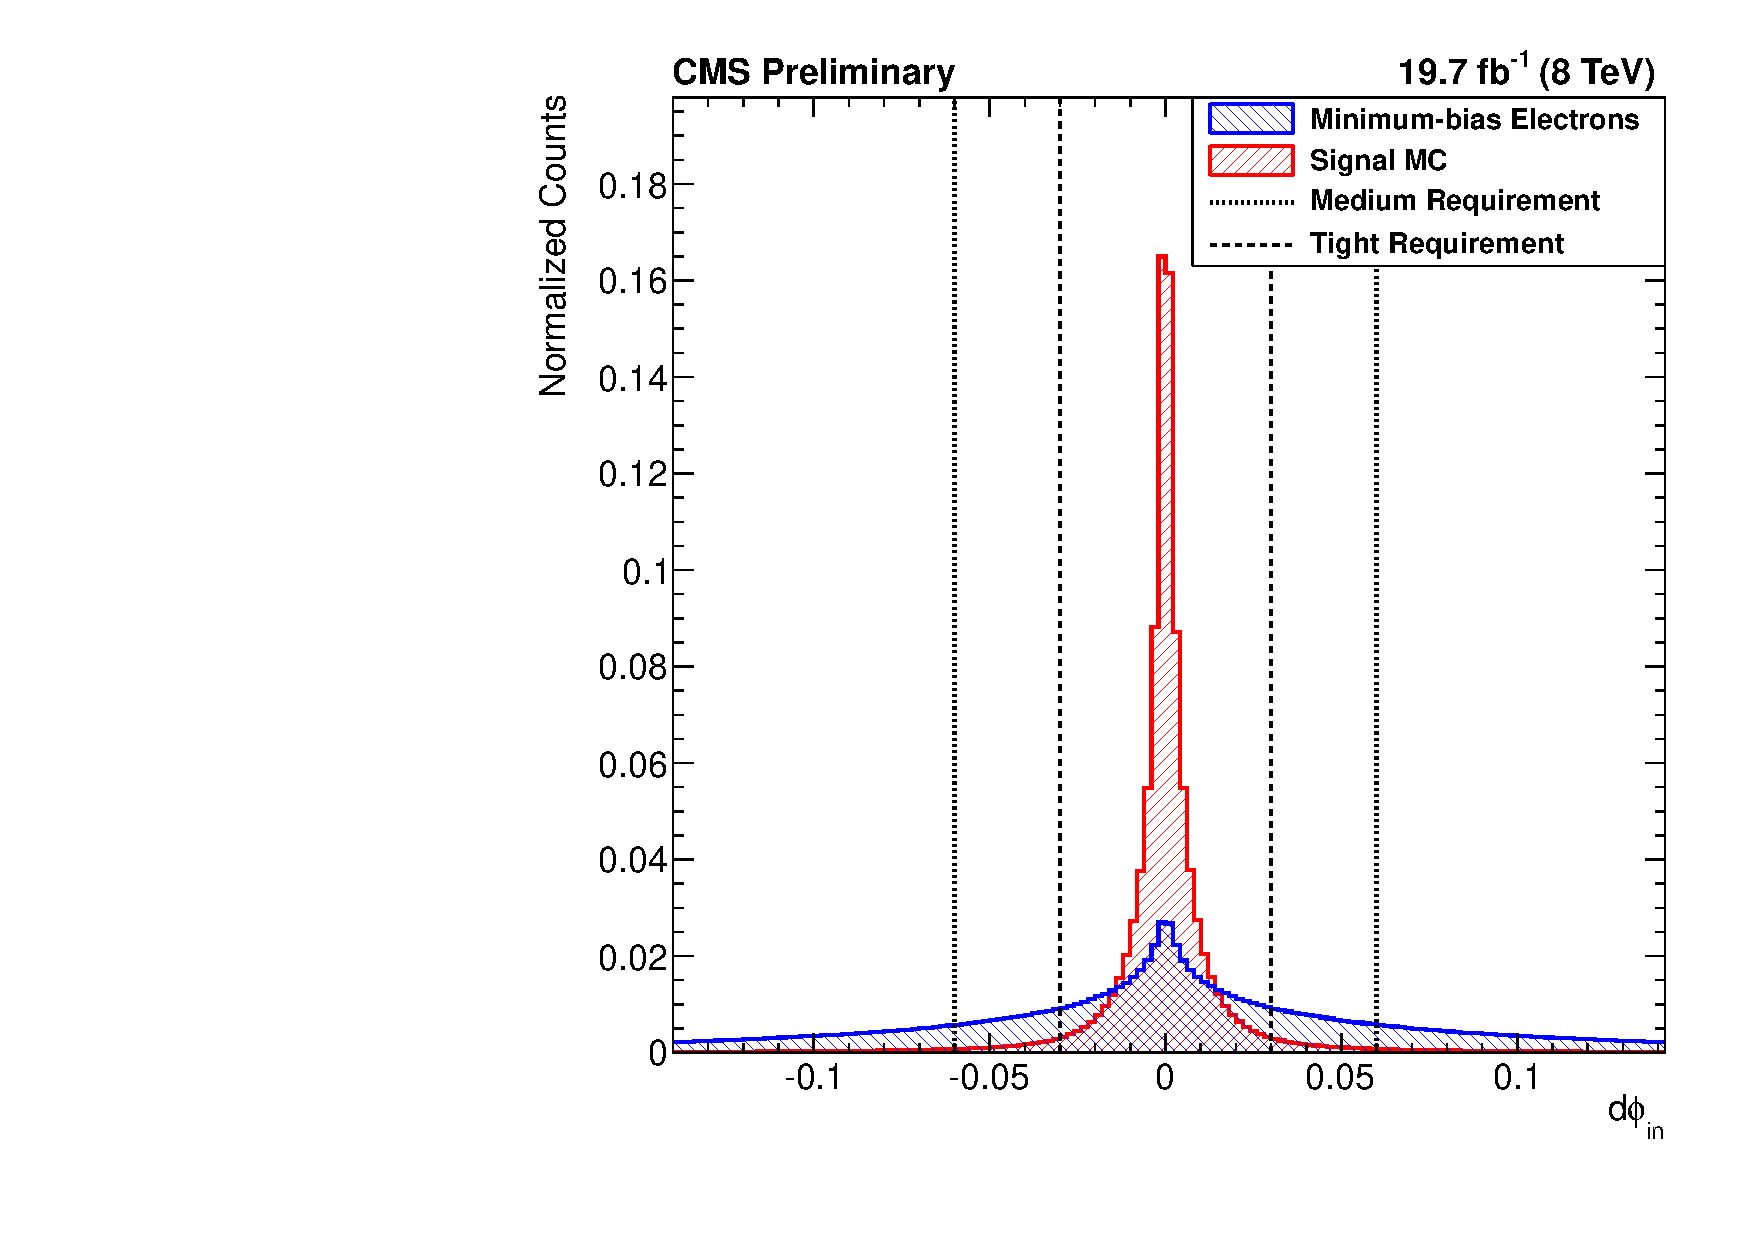
\includegraphics[width=\textwidth]{figures/e_reco_var_dphi.pdf}
        \caption{}
        \label{fig:dphi}
    \end{subfigure}
    \caption[
        Distributions of $\detain$ and $\dphiin$ in data and MC.
    ]{
        The $\detain$ (top) and $\dphiin$ (bottom) variable distributions for
        all electrons with $\pt > 20 \GeV$ and $|\eta| < 2.4$ in a set of
        events selected with a muon trigger and in \MADGRAPH \Ztoee MC.
    }
    \label{fig:dtrack}
\end{figure}

The compatibility of energy of the supercluster and the momentum of the track
is parameterized by \ooeoop. Electrons will have \ooeoop near \num{0} because
their momentum and energy, having been measured for the same object, will
agree. Charge exchange events will have positive \ooeoop as their momentum is
measured in the tracker before the interaction (and hence measures the full
momentum of the \pionplus) but their energy is measured in ECAL after the
interaction and hence after the proton has carried away some of the energy.
Coincidence events, because the energy and momentum are measured from
independent objects, can take both positive and negative values of \ooeoop. A
comparison of the \ooeoop distributions between all electrons and for signal
electrons is shown in \FIG~\ref{fig:ooeoop}.

\begin{figure}[!htbp]
    \centering
    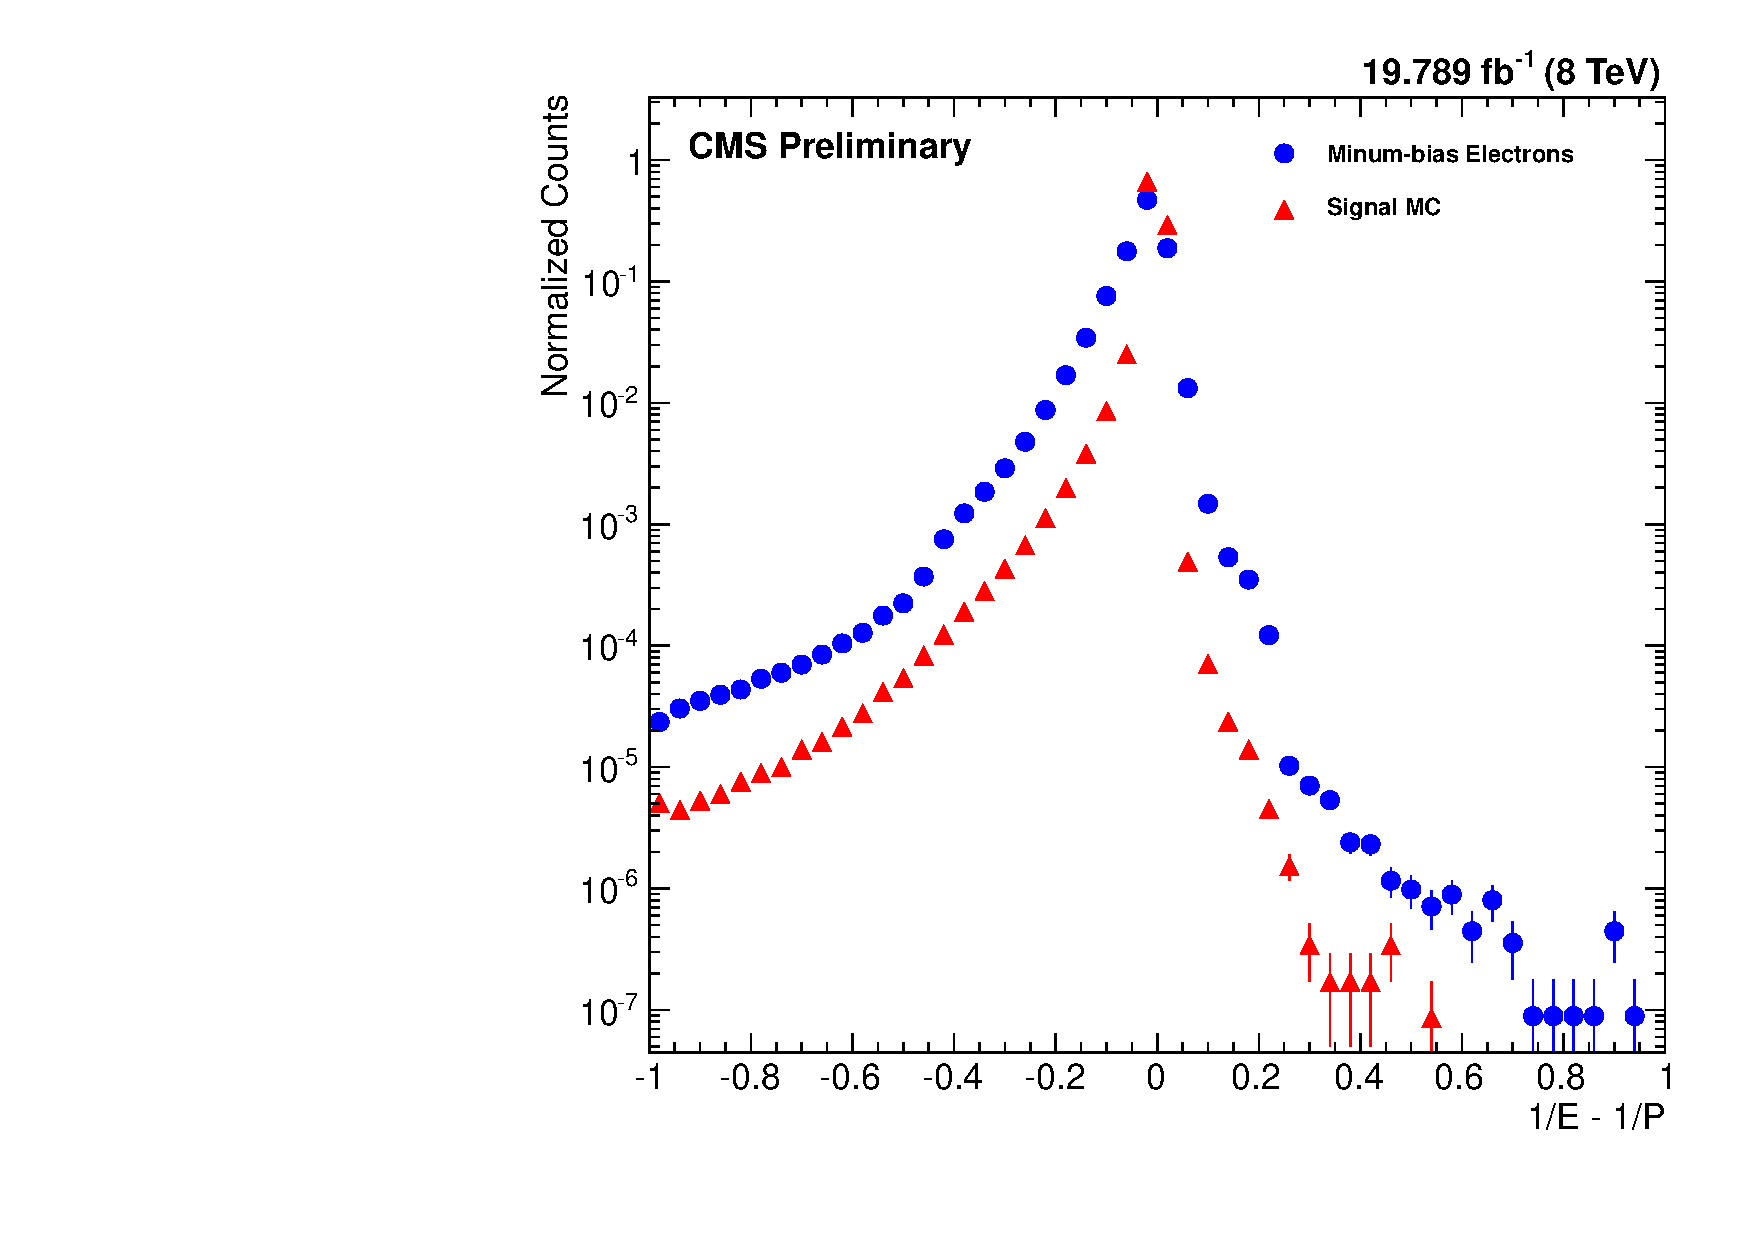
\includegraphics[width=\StackedPlotWidth]{figures/e_reco_var_1oe_1op.pdf}
    \caption[
        Distributions of \ooeoop in data and MC.
    ]{
        The \ooeoop distributions for all electrons with $\pt > 20 \GeV$ and
        $|\eta| < 2.4$ in a set of events selected with a muon trigger and in
        \MADGRAPH \Ztoee MC.
    }
    \label{fig:ooeoop}
\end{figure}

\subsection{Conversion Rejection}

Photon conversions generally happen away from the primary vertex and so the
distances of the hits in the track from the vertex are useful quantities to
reject conversions. The transverse and longitudinal separation between the
track and the primary vertex are given by \dzero and \dz. In addition to
the raw distance of the track from the primary vertex, there is also a fit
probability, \pvtx, which indicates the probability that a track came from the
primary vertex. This variable is also used to reject conversions. Comparisons
of the \dzero and \dz distributions between all electrons and for signal
electrons are shown in \FIGS~\ref{fig:d0} and \ref{fig:dz}, respectively.

\begin{figure}[!htbp]
    \centering
    \begin{subfigure}[b]{\StackedPlotWidth}
        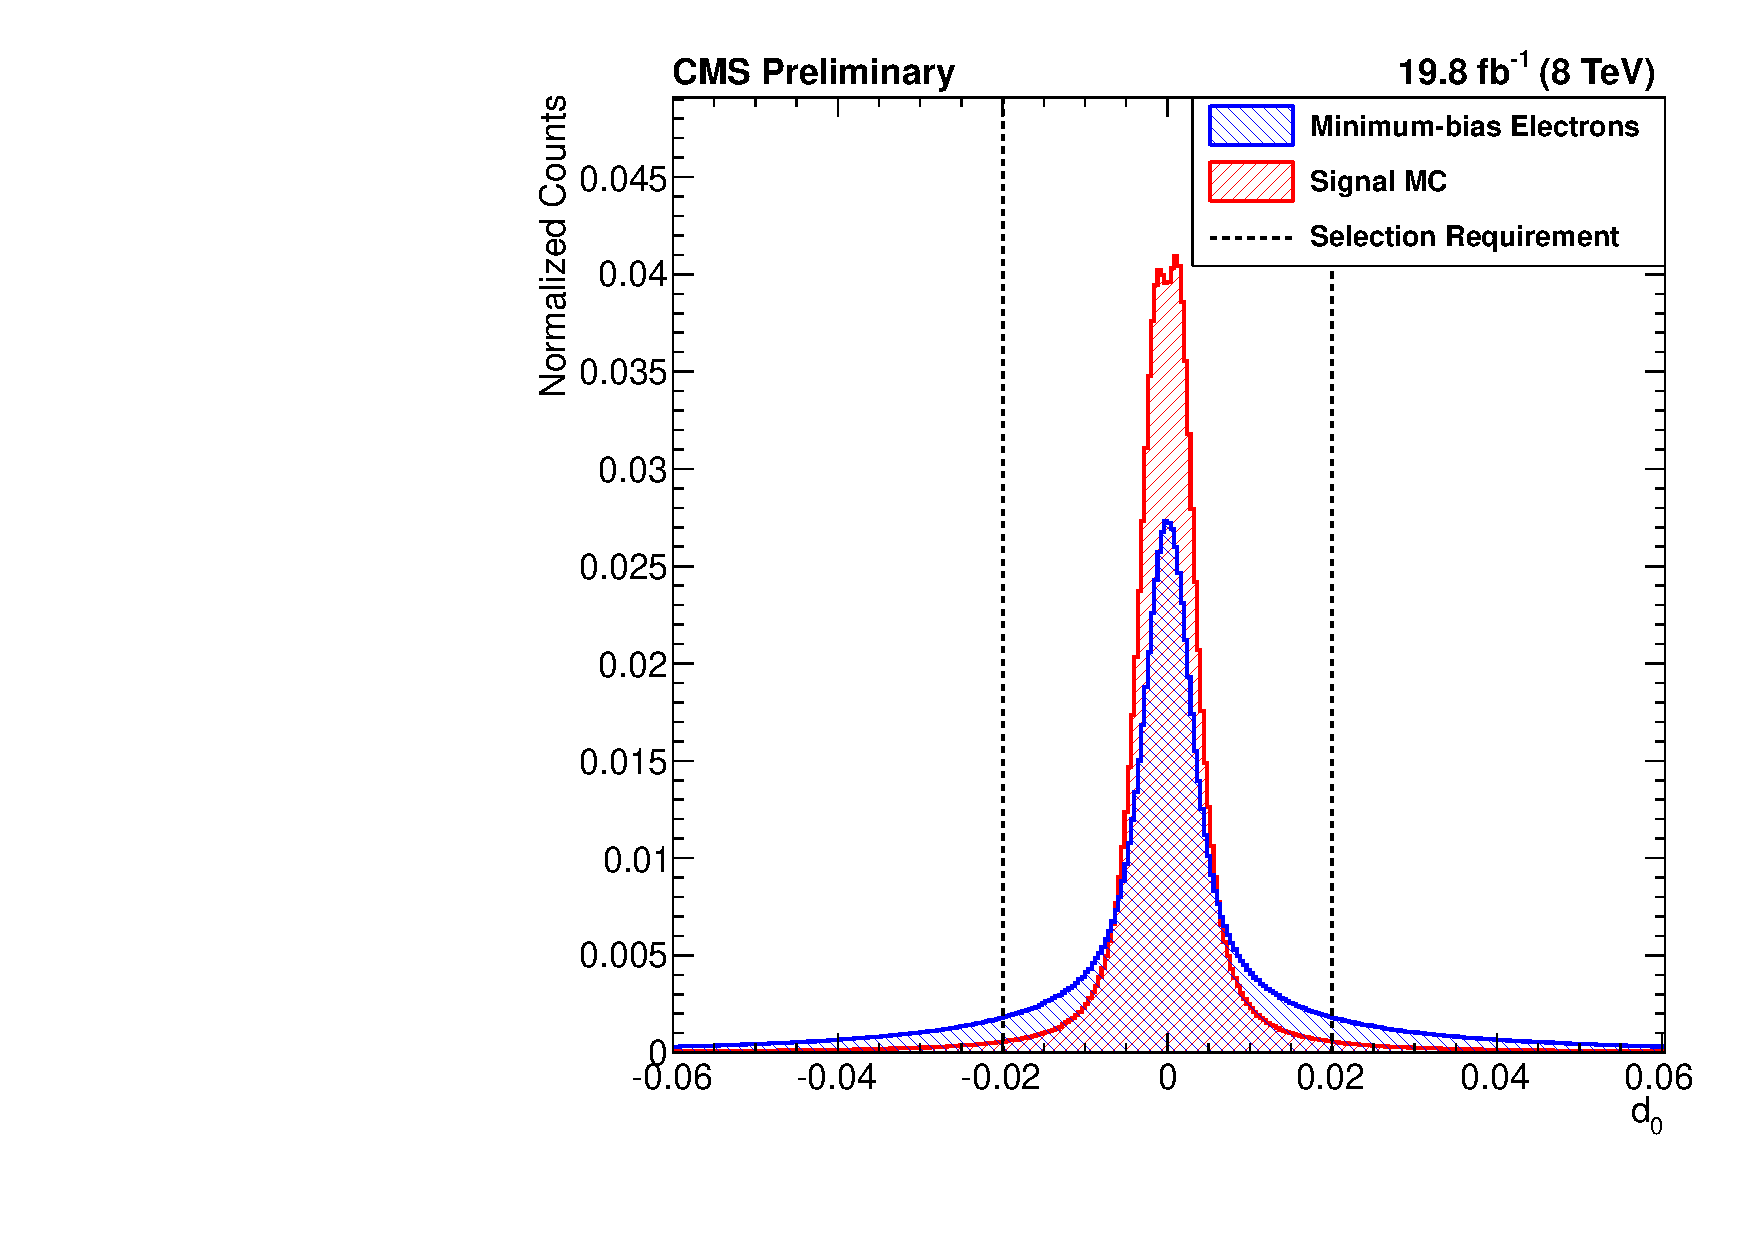
\includegraphics[width=\textwidth]{figures/e_reco_var_d0.pdf}
        \caption{}
        \label{fig:d0}
    \end{subfigure}
    \begin{subfigure}[b]{\StackedPlotWidth}
        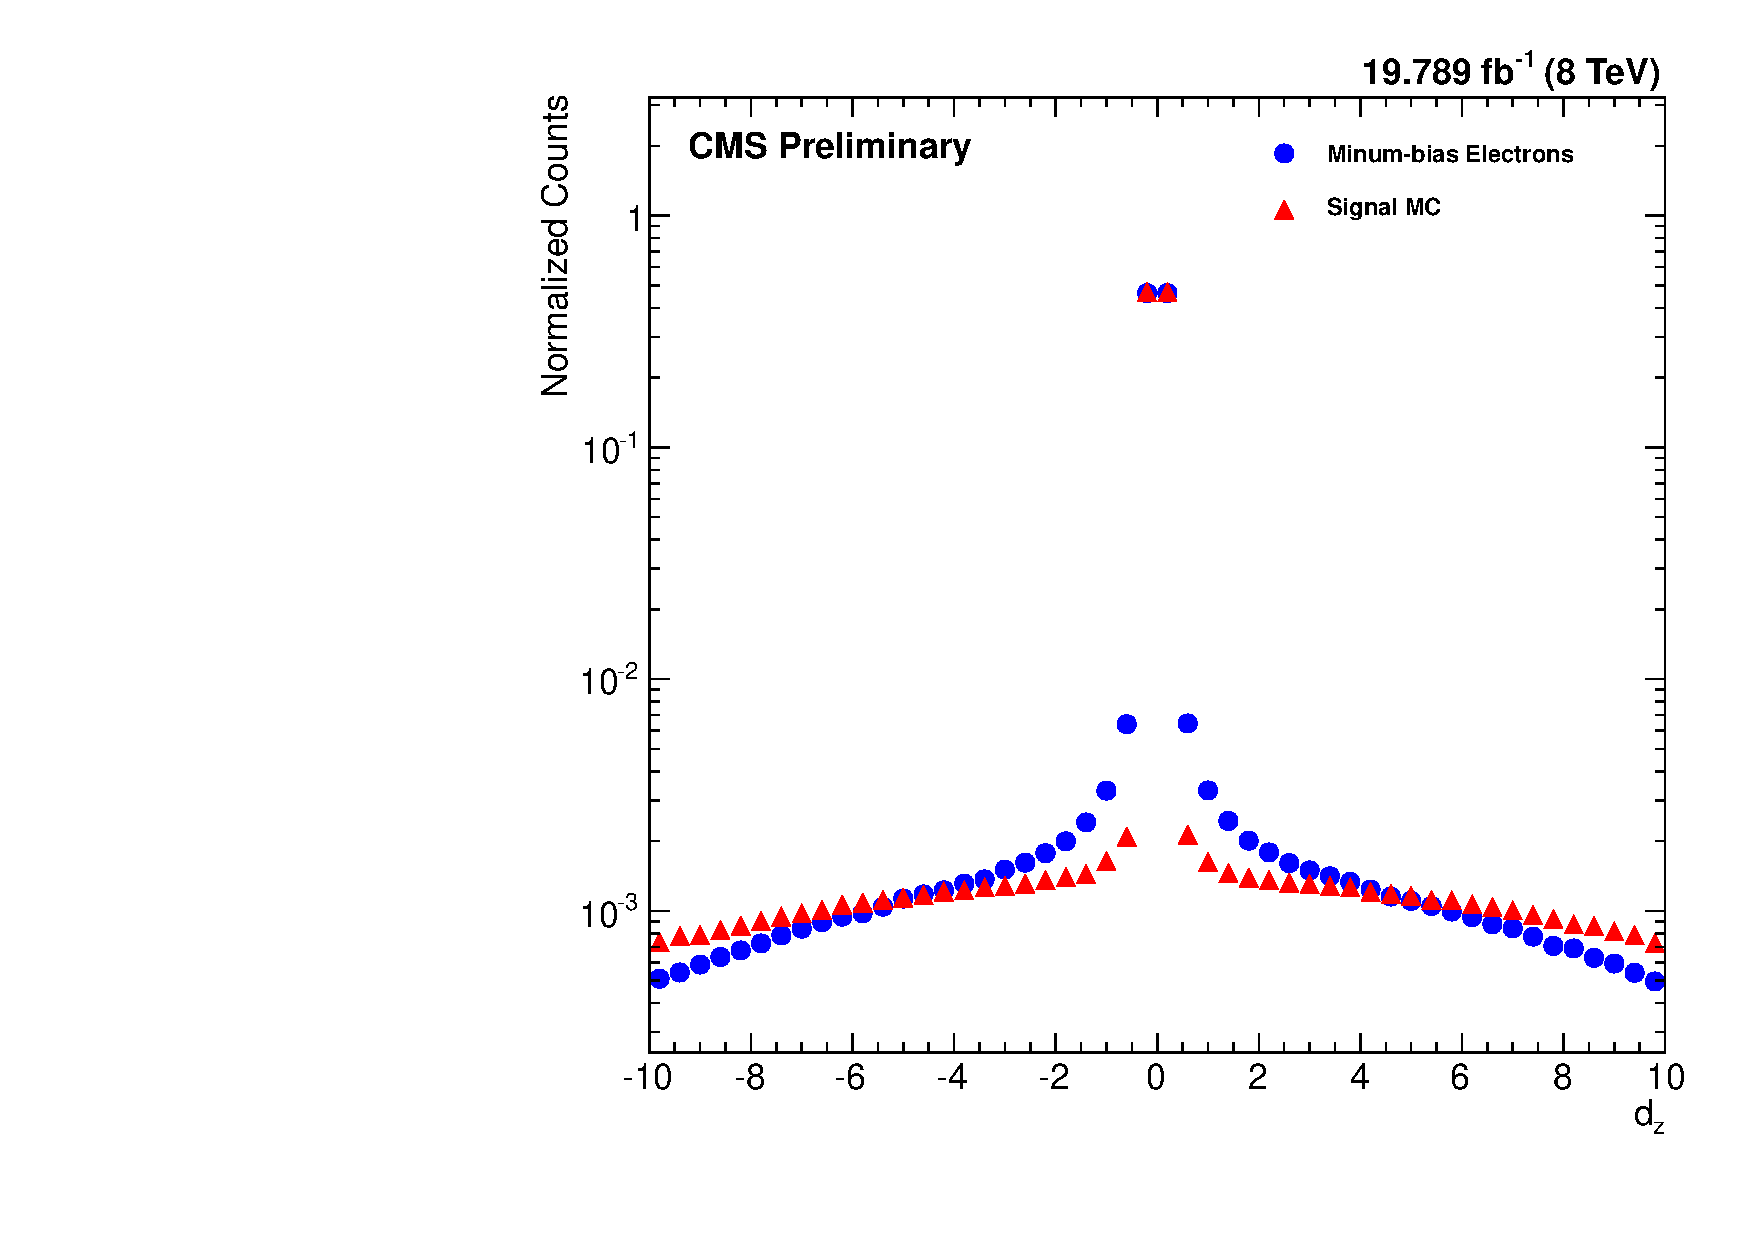
\includegraphics[width=\textwidth]{figures/e_reco_var_dz.pdf}
        \caption{}
        \label{fig:dz}
    \end{subfigure}
    \caption[
        Distributions of \dzero and \dz in data and MC.
    ]{
        The \dzero (top) and \dz (bottom) variable distributions for all
        electrons with $\pt > 20 \GeV$ and $|\eta| < 2.4$ in a set of events
        selected with a muon trigger and in \MADGRAPH \Ztoee MC.
    }
    \label{fig:d0_dz}
\end{figure}

Conversions generally happen after the photon passes through several layers of
the tracker and so their tracks will have missing layers, the number of which
is given by \nmiss. A comparison of the \nmiss distributions between all
electrons and for signal electrons is shown in \FIG~\ref{fig:nmiss}.

\begin{figure}[!htbp]
    \centering
    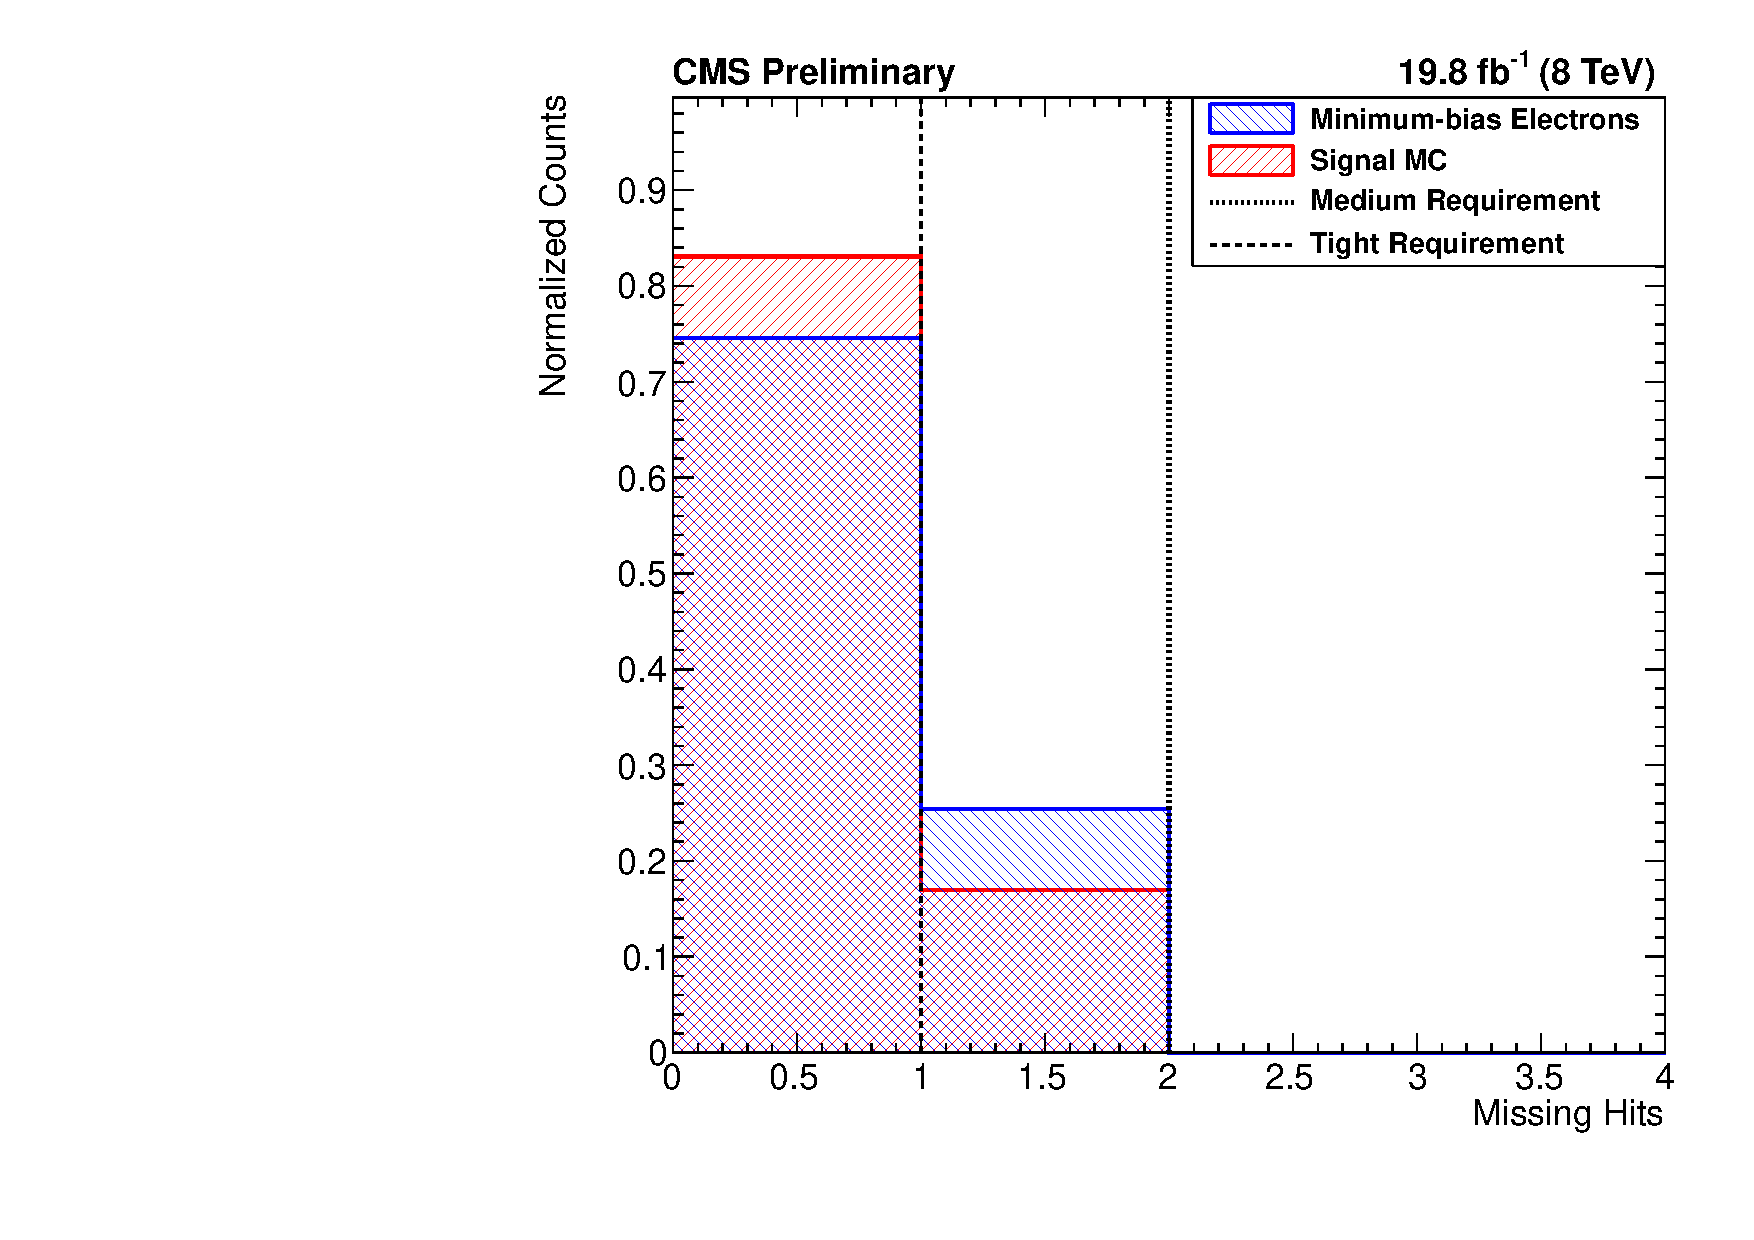
\includegraphics[width=\StackedPlotWidth]{figures/e_reco_var_nmiss.pdf}
    \caption[
        Distributions of \nmiss in data and MC.
    ]{
        The \nmiss distribution for all electrons with $\pt > 20 \GeV$ and
        $|\eta| < 2.4$ in a set of events selected with a muon trigger and in
        \MADGRAPH \Ztoee MC.
    }
    \label{fig:nmiss}
\end{figure}

\subsection{Isolation}

Hadronic jets sometimes produce electrons in the numerous decays happening
within them. These electrons can be rejected by looking at the sum of the
energy in the tracker, ECAL, and HCAL around the electron, as electrons in jets
will have a large amount of energy surrounding them, whereas electrons from \Z
decays will tend to be isolated.

The isolations used in the trigger (\SingleElectronTrigger) are defined as
follows:

\begin{equation}
    \HCALISO = \frac{\DeltaRSum \EHCAL}{\etElectron}
\end{equation}

\begin{equation}
    \ECALISO = \frac{\DeltaRSum \EECAL - \ESC}{\etElectron}
\end{equation}

\noindent where \DeltaRSum is a sum on the energy in a $\Delta R < 0.3$ cone around the
supercluster location, \EHCAL is the energy in HCAL, \EECAL is the energy in
ECAL, and \ESC is the energy of the supercluster, which is subtracted out of
the ECAL isolation sum. No subtraction is applied to the HCAL isolation as we
expect all of the electron's energy to be contained in ECAL. Both isolation
values are normalized by the \et of the electron. Comparisons of the \HCALISO
and \ECALISO distributions between all electrons and for signal electrons are
shown in \FIGS~\ref{fig:hcal_iso} and \ref{fig:ecal_iso}, respectively.

\begin{figure}[!htbp]
    \centering
    \begin{subfigure}[b]{\StackedPlotWidth}
        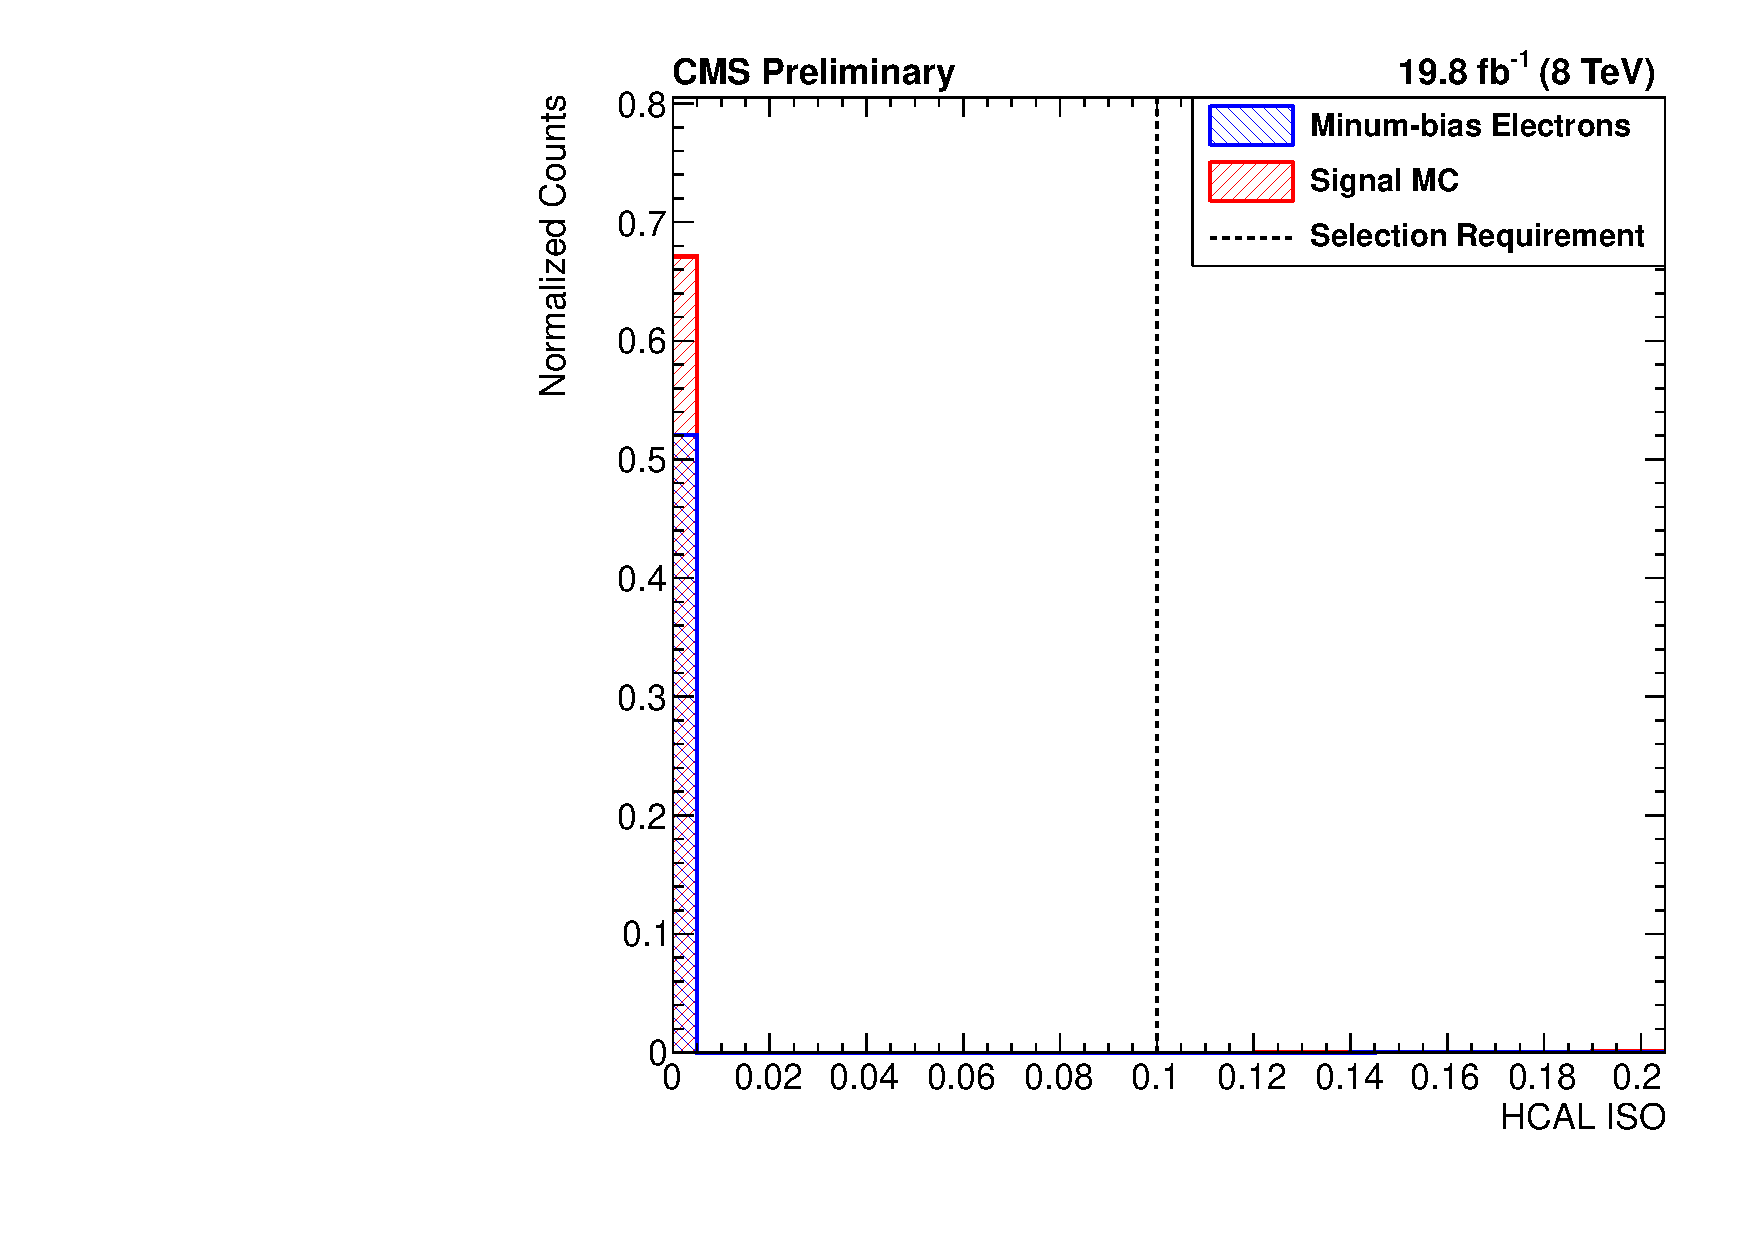
\includegraphics[width=\textwidth]{figures/e_reco_var_hcal_iso.pdf}
        \caption{}
        \label{fig:hcal_iso}
    \end{subfigure}
    \begin{subfigure}[b]{\StackedPlotWidth}
        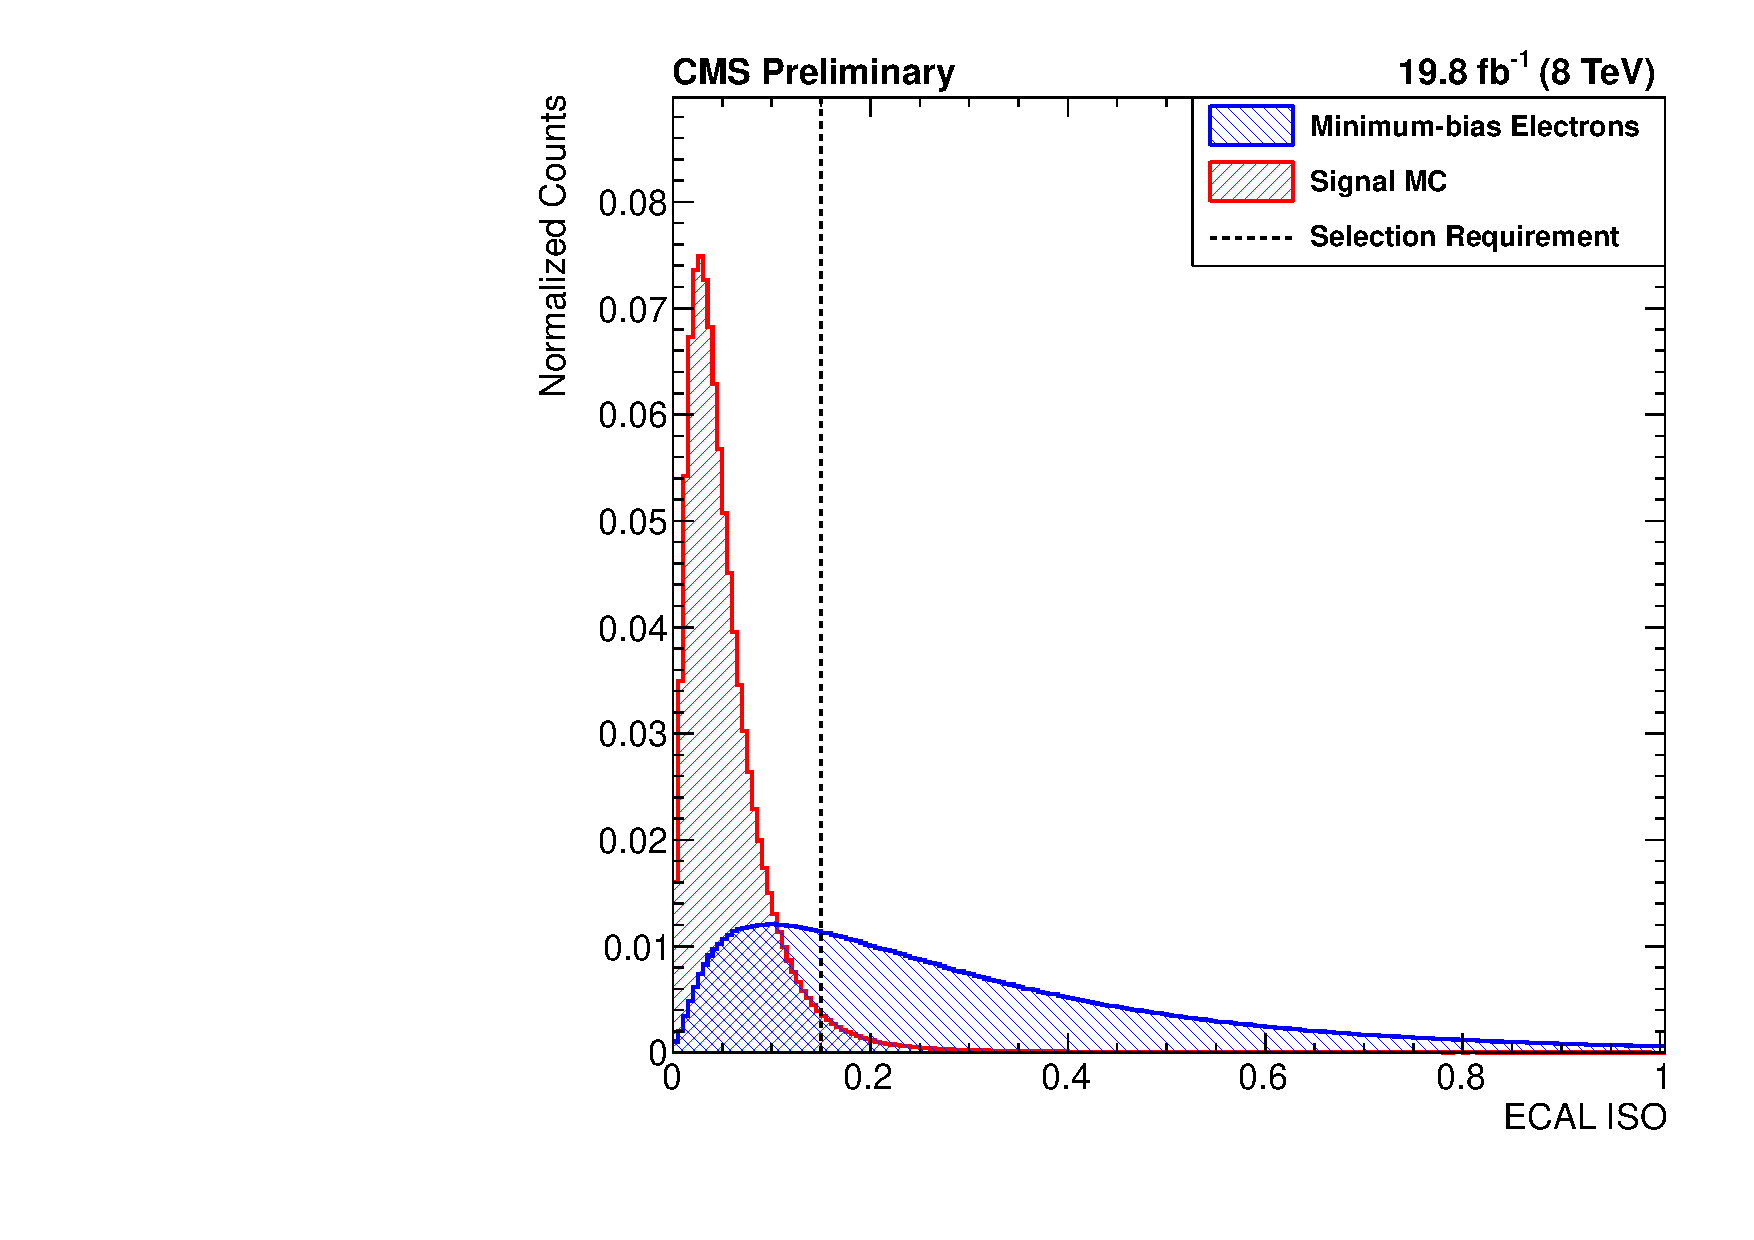
\includegraphics[width=\textwidth]{figures/e_reco_var_ecal_iso.pdf}
        \caption{}
        \label{fig:ecal_iso}
    \end{subfigure}
    \caption[
        Distributions of HCAL and ECAL isolation variables in data and MC.
    ]{
        The HCAL (top) and ECAL (bottom) isolation variable distributions for
        all electrons with $\pt > 20 \GeV$ and $|\eta| < 2.4$ in a set of
        events selected with a muon trigger and in \MADGRAPH \Ztoee MC.
    }
    \label{fig:hcal_ecal_isos}
\end{figure}

A different isolation variable is defined for selection of events in this
analysis that is more expensive to compute but takes advantage of the tracker
as well as ECAL and HCAL. This isolation uses a
``particle flow'' \cite{particle_flow_2009}\cite{particle_flow_2010} technique which
is a method of reconstructing jets that uses information for every subdetector
and tries to reconstruct the individual particles in a jet by matching them to
their responses in the various subdetectors. To keep the algorithm simple,
particle flow categorizes every particle into one of five types: photons,
electrons, muons, charged hadrons, and neutral hadrons. A photon is a particle
with energy only deposited in ECAL. An electron is a particle with an ECAL
energy deposit and a track. A muon is a track in the central tracker matched to
a track in the muon system. A charged hadron is any energy cluster in HCAL with
a possible matching ECAL cluster and track. A neutral hadron is any energy
cluster in HCAL with a possible matching ECAL cluster without a matching track.
These particle flow jets are used to calculate an energy density due to pileup,
$\rho$, in the detector which is used to remove the pileup contribution from
the isolation sum. The particle flow isolation, $\PFISO$, is given by:

\begin{equation}
    \PFISO = \DeltaRSum \frac{\left(\ptTrack + \EECAL + \EHCAL\right) - \ptElectron
    - \ESC - 0.3^{2} \pi \rho}{\ptElectron}
\end{equation}

\noindent where the variables are the same as above, with the addition of \ptTrack, which
is the \pt of all tracks in the tracker, \ptElectron, which is the \pt of the
electron's track, and $\left(0.3^{2} \pi \rho\right)$, which is the energy
around the electron due to pileup calculated from particle flow. The
particle flow isolation is normalized by the \pt of the electron. A comparison
of the \PFISO distributions between all electrons and for signal electrons is
shown in \FIG~\ref{fig:pf_iso}.

\begin{figure}[!htbp]
    \centering
    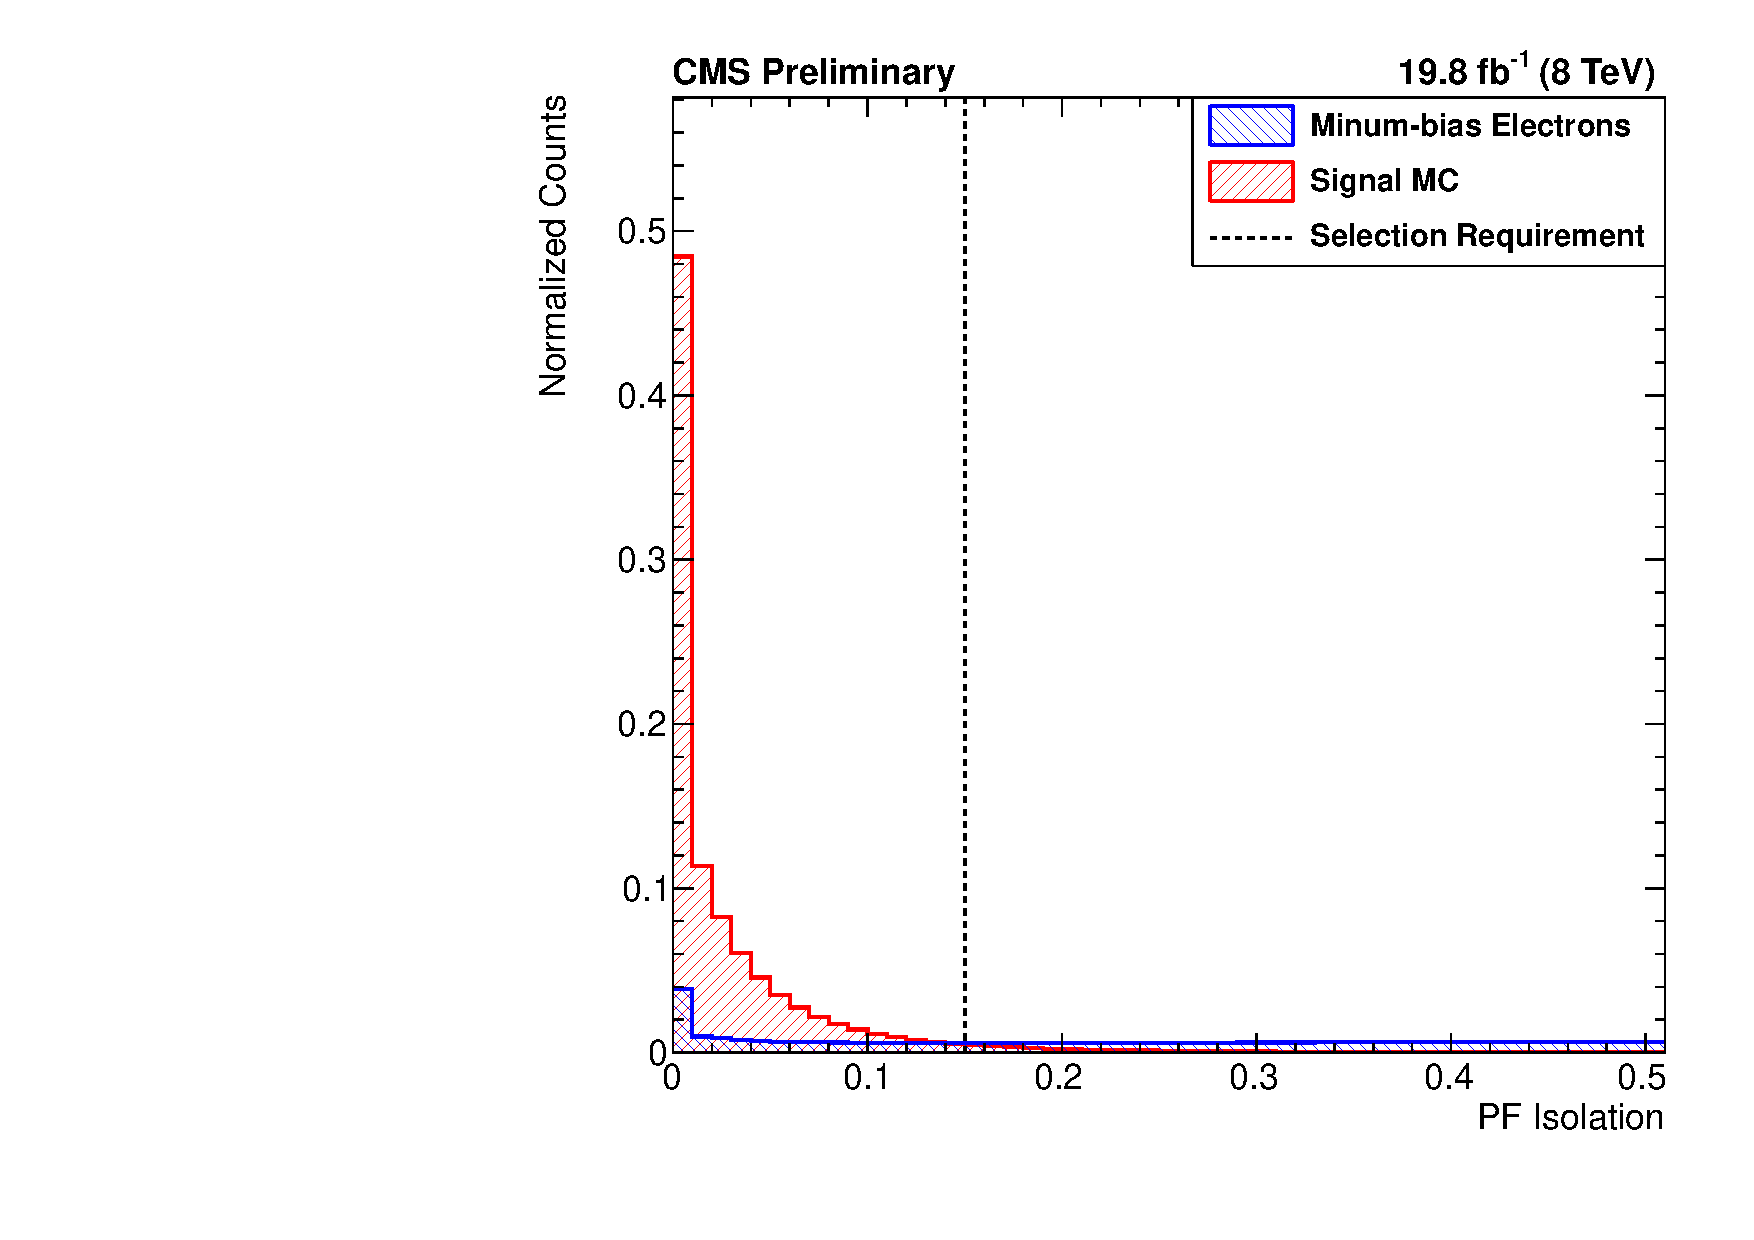
\includegraphics[width=\StackedPlotWidth]{figures/e_reco_var_iso.pdf}
    \caption[
        Distributions of particle flow isolation variables in data and MC.
    ]{
        The particle flow isolation variable distribution for all electrons
        with $\pt > 20 \GeV$ and $|\eta| < 2.4$ in a set of events selected
        with a muon trigger and in \MADGRAPH \Ztoee MC.
    }
    \label{fig:pf_iso}
\end{figure}

\section{Cut Based Identification}
\label{sec:cut_based_id}

There are several centrally-defined ``cut based identification'' requirements
used to select high quality electrons at CMS. These requirements make use of
the variables defined in \SEC~\ref{sec:electron_variables} in order to reject
low quality and unisolation electrons. We use two of requirements, referred to
as \EGMEDIUM and \EGTIGHT, with \EGTIGHT having stricter requirements than
\EGMEDIUM. The exact definition of these requirements are given in
\TAB~\ref{table:eg_cuts}.

% table:eg_cuts
\begin{table}[h]
    \centering
    \spacerows{1.2}
    \begin{center}
        \begin{tabular}{@{}l r r r r r@{}}
            \toprule
            \multirow{2}{*}{Variable}     & \multicolumn{2}{c}{\EGTIGHT} & \phantom{abc}   & \multicolumn{2}{c}{\EGMEDIUM} \\
            \cmidrule{2-3}
            \cmidrule{5-6}
            & \multicolumn{1}{c}{EB} & \multicolumn{1}{c}{EE} && \multicolumn{1}{c}{EB} & \multicolumn{1}{c}{EE} \\
            \midrule
            $\detain <$                   & 0.004     & 0.005     && 0.004     & 0.007 \\
            $\dphiin <$                   & 0.03      & 0.02      && 0.06      & 0.03 \\
            $\sigmaietaieta <$            & 0.01      & 0.03      && 0.01      & 0.03 \\
            $\HOverE <$                   & 0.12      & 0.10      && 0.12      & 0.10 \\
            $\dzero <$                    & 0.02      & 0.02      && 0.02      & 0.02 \\
            $\dz <$                       & 0.1       & 0.1       && 0.1       & 0.1 \\
            $|\ooeoop| <$                 & 0.05      & 0.05      && 0.05      & 0.05 \\
            $\pvtx <$                     & $10^{-6}$ & $10^{-6}$ && $10^{-6}$ & $10^{-6}$ \\
            $\nmiss \le$                  & 0         & 0         && 1         & 1 \\
            $\PFISO <$                    & 0.10      & 0.10      && 0.15      & 0.15 \\
            \bottomrule
        \end{tabular}
    \end{center}
    \caption[
        Identification and isolation requirements for \EGTIGHT and \EGMEDIUM.
    ]{
        Identification and isolation requirements for \EGTIGHT and \EGMEDIUM
        requirements in the ECAL barrel (EB) and ECAL endcap (EE).
    }
    \label{table:eg_cuts}
\end{table}

